\documentclass{intech}
 
%\usepackage{your_package}	%if you need custom package
%\usepackage[notquote]{hanging}
 

% * CHAPTER NUMBER * BOOK NAME * AUTHOR(S) NAME *****************************
\setcounter{chapter}{0} % It will be set by technical editor.

\booktitle{Wireless Energy Transfer  based on Electromagnetic Resonance: Principles and Engineering Explorations}%

\chaptertitle{The Phenomenon of Wireless Energy Transfer: Experiments and Philosophy} % You know your chapter title?

\authors{H. V\'azquez-Leal, A. Gallardo-Del-Angel, R. Casta\~neda-Sheissa and F. J. Gonz\'alez-Mart{\'i}nez}
\affiliation{Universidad Veracruzana \\ Facultad de Instrumentaci\'on Electr\'onica}
\country{M\'exico}

% uncomment the next three or six lines, when authors are from diferent university, company or country

%\secondauthors{Author(s) with another affiliation}
%\secondaffiliation{Name of the 2nd University (Company)}
%\secondcountry{2nd country}

%\thirdauthors{}
%\thirdaffiliation{}
%\thirdcountry{}

% END * CHAPTER NUMBER * BOOK NAME * AUTHOR(S) NAME *************************


\begin{document}

\maketitle

\section{Introduction}

There is a basic law in thermodynamics; the law of conservation of energy, which states that {\it energy may neither be created nor destroyed just can be transformed}. Nature is an expert using this physics fundamental law favoring life and evolution of species all around the planet, it can be said that we are accustomed to live under this law that we do not pay attention to its existence and how it influence our lives.

At the present time, wireless energy transfer has gained importance, that is energy distribution without cables. Nevertheless, nature has always been a step beyond us, doing energy distribution and transformation {\it since a long while} without the need of copper cables. The biggest wireless transfer source known is solar energy; nature uses sunlight to drive the photosynthesis process, generating this way nutrients that later on will become the motor for the food chain and life. Nowadays, several ways to turn sunlight into electrical power have been invented, among them, the photo-voltaic cells are the most famous. However, a new technological tendency seeks to transfer energy by wireless means from point to supply the energy to charge mobile devices immediately, or provide power to biomedical implants among other applications. In fact, this new technology tendency towards wireless energy is not really new as one might think. In early 19th century a scientist named Nikola Tesla performed experiments (\cite{RES20}) on wireless energy achieving amazing results for his time. Nevertheless, perhaps by the dangerous nature of the experiments, the low efficiency on the transfer and the lack of interest on the people o its skepticism, Tesla dropped the experiments leaving his legacy in a way of a patent that was never commercially developed.

Electromagnetic radiation has been employed, typically, for wireless information transfer. Nonetheless, information travels on electromagnetic waves which is an energy form. Therefore, theoretically it is possible to transfer energy in a similar way to transfer information (voice and data). In particular, it is possible to transfer huge amounts of energy in a certain direction using microwaves ({\cite{RES22}). Although the method is efficient, it has two drawbacks: requires a line of sight and is a dangerous mechanism for living creatures. Hence, wireless energy transfer (\cite{RES1}) by means of resonant coupling has become a viable option, at least for short distances, because is not dangerous and provides good efficiency.

%En \'epocas recientes diversos investigadores han tratado de transferir energ{\'i}a de forma inal\'ambrica usando diversos mecanismos f{\'i}sicos como lo son: rayo laser(\cite{RES21}), 
%principio piezoel\'ectrico(\cite{RES8}), ondas de radio y microondas (\cite{RES22,RES4,RES9}) y acoplamiento inductivo (\cite{RES3,RES5,RES6,RES7}).



\section{Acoustic and Electric Resonance}

The mechanical resonance or acoustic is well known on physics and consists in applying to an object a vibratory periodic action with a vibratory period that match the maximum absorption energy rate of the object. That frequency is known as resonant frequency. The phenomenon well known in mechanics is also present in electricity and is called electrical resonance or inductive. Such phenomenon can be used to transfer wireless energy with two main advantages: maximum absorption rate is guaranteed and it can work in low frequencies (less dangerous to humans). When two objects have the same resonant frequency, they can be coupled in a resonant way causing one object to transfer energy (in an efficient way) to the other.

Here three wireless power transmission mechanisms are described:
\begin{enumerate}
\item {\bf Inductive coupling (\cite{RES3})} is a resonant coupling that takes place between coils of two $LC$ circuits with the same resonant frequency, transferring energy from one coil to the other as it can be seen in figure \ref{fuerte}. The disadvantage of this technique is that efficiency is lost as fast as coils are separated.
\item {\bf Self resonant coupling (\cite{RES1})}. The self resonance occur in a natural way for all the coils ($L$), although the frequency ($f_r=1/(2\pi \sqrt{L C_p})$) is usually too high because the parasitic capacitance ($C_p$) value is too low. Nevertheless, in (\cite{RES1}) was shown that it is possible to achieve good efficiency with a scheme like the one shown in figure \ref{fuerte}(b). There are two fundamental differences for the simple inductive coupling in figure \ref{fuerte}(a), those are: the capacitance of the $LC$ circuit is parasite, not discrete, and now coils ($T$ y $R$) are coupled to two one spire coils $L_S$ and $L_L$, those act as the emitter source and receiver coils, respectively. The coil's self resonant frequency depends of its parasite capacitance, that is the reason the frequency is very high (around the GHz range). Therefore, to achieve lower self resonance frequency ($<10$Mhz) it is necessary to use thick and spaced copper wire to create higher parasite capacitance, reducing the self resonance frequency down to the megahertz range. In fact, in \cite{RES1} and \cite{RES2} is reported an experiment using cable with radius $>1$ cm. The efficiency on the power transfer with respect to the distance has an inverse relationship to the radius of the coil, that is why the experiments reported in \cite{RES1} and \cite{RES2} coils have 30 cm. radius.
\item In figure \ref{fuerte}(c), the coupling scheme shown can be named as {\bf modified resonant inductive coupling}, this is a modification for the strong resonant coupling (see figure \ref{fuerte}(b)). The modification consists in exchange the parasite capacitance $C_p$ for a discrete capacitance $C$. Thus, the need for large and thick cable is eliminated.
\end{enumerate}

\begin{figure}[htbp]	% H-must be here or [htb]
\centering
\subfigure[Inductive resonant coupling]{\includegraphics[width=3.7cm]{./img/acoplamientos-1.eps}} %	** if .eps don't need extension
\hspace{0.5cm}
\subfigure[Strong self-resonant coupling]{\includegraphics[width=3.7cm]{./img/acoplamientos-2.eps}}
\hspace{0.5cm}
\subfigure[Modified inductive resonant coupling]{\includegraphics[width=4cm]{./img/acoplamientos-3.eps}} %	** if .eps don't need extension
\vspace{-0.5cm}
\caption{Coupling schemes}
\label{fuerte}
\end{figure}

\section{Experimentation}
The purpose of the experimentation stage is to compare the three schemes shown in figure \ref{fuerte}. The experiments are described in the following:
\vspace{-0.3cm}
\begin{enumerate}
\item {\bf Inductive resonant coupling}. This experiment was designed (\cite{SOMI}) to visualize the radiation pattern and the efficiency of an inductive resonant coupling. First, the generating coil was kept in a fixed position while the receiver coil ($R$) revolves around the generating coil ($T$), at a fixed distance and with constant angular displacement completing 360 degrees (see figure \ref{datos1}(a)). The experiment shows that the produced energy by the transmitter coil $T$ propagates at 90$^\circ$ in front of the generating coil and at 90$^\circ$ behind the same coil. In another stage of the experiment, two coils were placed in parallel and concentric at a distance of zero centimeters, then they were moved away. The results are shown in figure \ref{datos1}(b). It can be seen from figure \ref{datos1}(c) that the maximum efficiency for voltage gain is around the 50\% (at zero centimeters). The result is logical after observing  the radiation pattern shown in figure \ref{datos1}(b), because a radiation back lobe is wasted. Figure \ref{datos1}(c) shows, beyond the 8 cm distance, the voltage gain for the system falls below the 5\% value. The back lobe could be reused using a reflecting surface for the magnetic field.

\begin{figure}[htbp]	% H-must be here or [htb]
\centering
\subfigure[Experimental process for the revolving coil]{\includegraphics[width=5cm]{./img/coil3d.eps}} %	** if .eps don't need extension
\subfigure[Radiation pattern]{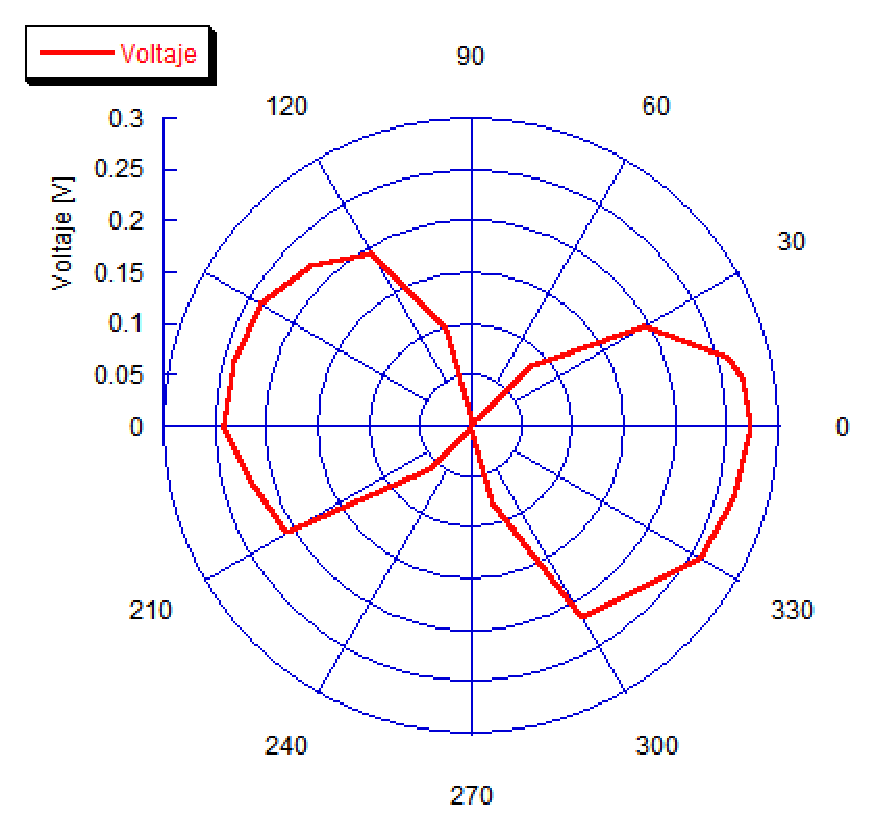
\includegraphics[width=4cm]{./img/image1a.eps}}
\subfigure[Voltage gain of the system with respect to the voltage ratio]{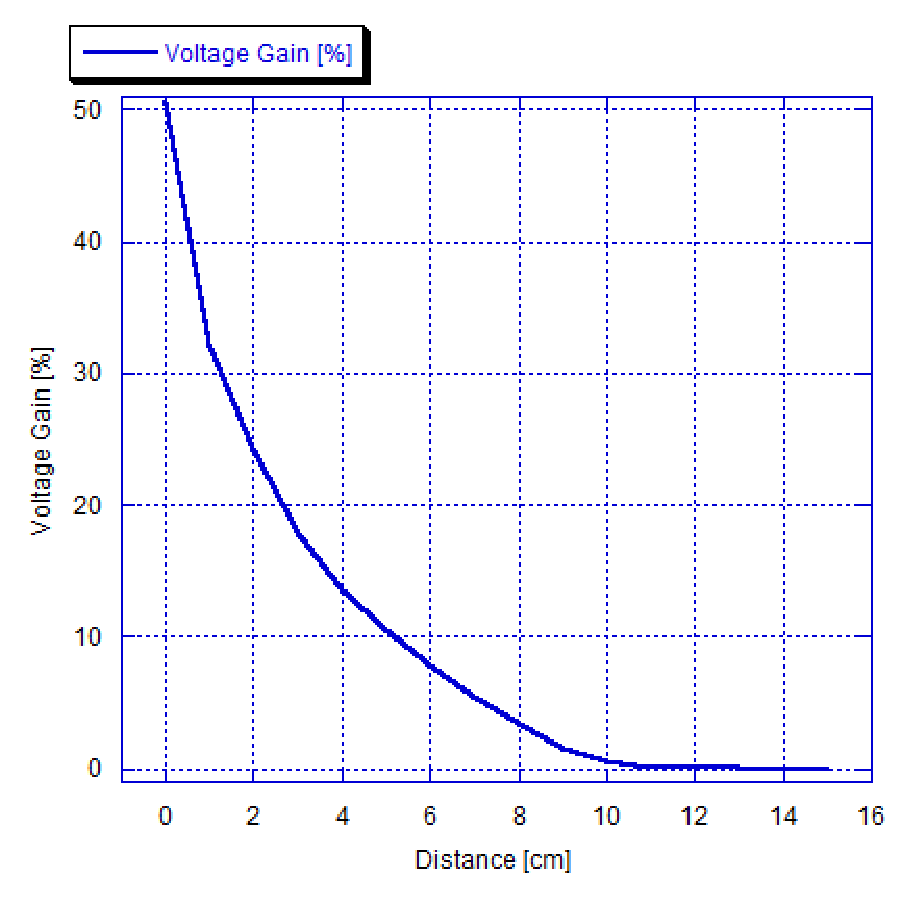
\includegraphics[width=3.5cm]{./img/image2.eps}} %	** if .eps don't need extension
\vspace{-0.3cm}
\caption{Generator coil radiation pattern.}
\label{datos1}
\end{figure}
\item  {\bf Modified resonant inductive coupling}. In the complete version of this work, the results will be presented.
On this experiment the previous procedure will be repeated, but the scheme employed is shown in figure \ref{fuerte}(c). The results obtained and the following discussion will be presented in the complete document, also a comparison to the experiment 1 will be included.
\item  {\bf Triangular coil}. At this moment preliminary results are being gathered and on review.  In the complete version of this work, the results will be presented.


\item {\bf Waveguide}. Experiments 1 and 2 will be repeated using a waveguide for the transmitter coil and a reflecting stage for the back lobe of the radiation pattern. The expected result is the achievement of higher efficiency at grater distance.
\end{enumerate}
\section{Philosophy}
The wireless energy with: high power (>100W), reaching longer distance (>10m), having good efficiency (>70\%), without health concerns, and low cost is a dream that keeps the attention of researchers around the planet. Nevertheless, in order to make a dream come true it is necessary innovating ideas or even radical ones, to provide the answer for the big questions opposed to achieve the goal. Therefore, innovation is required on the following directions:

\begin{itemize}
\item Coils with different geometries. Coils employed on the reported experiments are just a single spiral.  Nevertheless, new geometries (triangular, hexagonal, multiform) can be used and thus modify the radiation pattern, this modification on the pattern seeks the increase of: directionality, distance and/or efficiency.

%like the ones shown in figure \ref{patronloco}.




%\begin{figure}[hbtp]
%\centering
%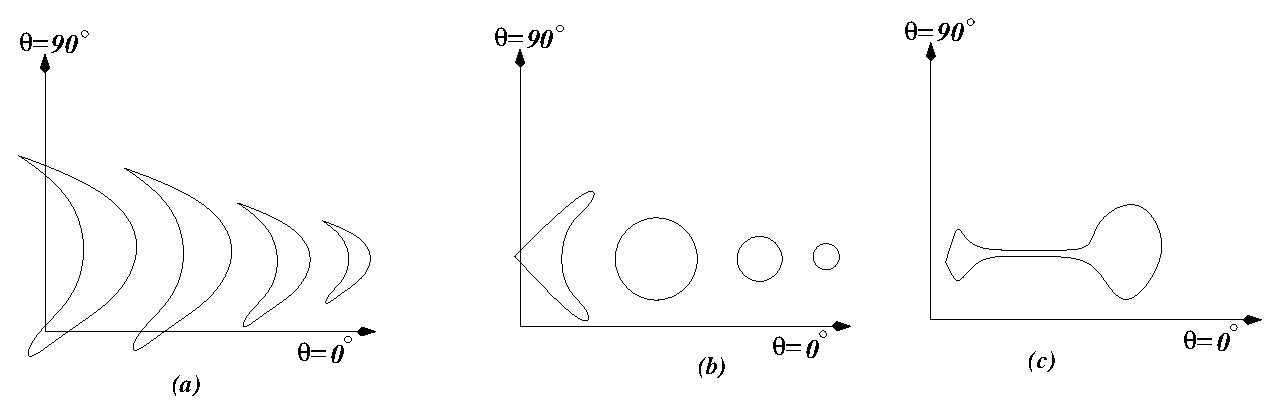
\includegraphics[width=12cm]{img/patrones.eps}
%\caption{New radiation patterns}
%\label{patronloco}
%\end{figure}
\item Using new materials to improve efficiency. For instance, from the self-resonance coils in experiment 2, it can be achieved using a coil-capacitor device. This coil could be designed in such a way that between each spire a dielectric material is placed to create parasite capacitance along all the coil spires. Therefore, parasite capacitance will be big enough to achieve self-resonance on the order of MHz. The advantage of this coil-capacitor is that no longer thick coils and spaced spires will be needed.
%\item Arreglos de bobinas. Se colocar{\'i}an pequeñas bobinas en arreglos especiales con la finalidad de sumar campos electromagn\'eticos, creando as{\'i} nuevos patrones de radiaci\'on.
\item Inductive coupled multi-resonant systems. Using amorphous or multiform coils could generate multiple resonant frequencies that could be employed in the transfer of energy using more than one resonant frequency, this will depend on their emitting pattern and efficiency extent. Another possible application for multi-resonant systems is transmission of energy and information a the same time using different channels. For instance, using the information channel to establish the permission for the energy transfer and features like power levels.
\end{itemize}


\bibliography{lrc}

\end{document}
